\documentclass[11pt]{jarticle}
\usepackage{ITCannual}
\usepackage{amsmath}
\usepackage{amssymb}
\usepackage{times}
\usepackage{graphicx}

%\usepackage[style=numeric]{biblatex}

\title{データ科学研究部門 研究報告}
\author{小林, 松島, 姜, 川瀬}

\begin{document}
\maketitle

\section{前年同様、各部門自由記述}
...

\section{データ科学部門の研究活動}

\subsection{研究報告(小林)}


\subsection{研究報告(松島)}
本節では松島研究室の研究活動について報告する。
2019年度および2020年度に、弊研究室では解釈可能な機械学習手法の効率的な計算手法についての研究を推進してきた。

画像データや言語データを予測したり生成したり表層的に駆使することは可能になってきた。
しかしながら我々の画像や言語の理解が進んだわけではない。

機械学習は予測や分類など表層的なデータの駆使の方法論であるだけでなく、
データの関係を明らかにして人間の理解を助けるための方法論でもある。

特にデータ保持者の目線に立って機械学習を


成果は主に以下の3分野に大別される。
\begin{itemize}
    \item 一般化加法モデルに関する研究
    \item 組合せ線形モデルに関する研究
    \item 部分空間クラスタリングに関する研究
\end{itemize}

一般化加法モデルと組み合わせ線形モデルは
属性間の線形な関係を越えて、非線形な関係を抽出するための枠組みである。
部分空間クラスタリングはデータ集合が持つ単純な線形関係を超えて、
データのクラスタリングを行ってそれぞれのクラスタが持つ線形関係を抽出する枠組みである。


\subsubsection{一般化加法モデルに関する研究}
いわゆる線形モデルの学習とは以下のようにあらわされる
データの属性間の線形な関係を抽出する枠組みととらえることができる
\begin{align*}
    y = \sum_{j} w_j x_j
\end{align*}
データの属性$y$は通常予測したい変数であり、
他のデータ属性が$x_j$である。与えられたデータ集合を用いて$w_j$は実数全体から推定される。
一般化加法モデルでは以下のような関係を抽出する枠組みである
\begin{align*}
    y = \sum_{j} f_j (x_j)
\end{align*}
与えられたデータ集合を用いて$f_j$は(十分広い)関数クラス$F$から推定される。
このような$f_j$を推定できれば、例えば年齢と収入の非線形な関係などがデータから
学習できると考えられる。

最も単純な手法は$F$を推定の簡単さのために狭めの関数クラスに制限することである。
一般に与えられた基底関数集合$\left\{\varphi_k(\cdot):\mathbb{R} \to \mathbb{R} \right\}_{k=1,\ldots,K}$に対し
\begin{align*}
  F=\left\{  \sum_{k=1}^d \varphi_k(x_j) \right\}
\end{align*}
とすることはパラメトリックな手法と呼ばれる。
\cite{F}は〜\\

利用可能なデータ数に応じて関数クラスの大きさが変わる。
具体的にはデータ数が大きくなれば関数クラスも広くなっていくような手法をノンパラメトリックな手法と呼び、
そのような手法はカーネル法を使うよりなかった。
我々の手法はカーネル法よりも効率的に学習が可能である。


さらに複雑な関係性をデータから学習して可視化することが可能である
\begin{align*}
    y = \sum_{j,k} f_{j,k} (x_j,x_k)
\end{align*}




\subsubsection{組合せ線形モデルに関する研究}

組合せ線形モデルでは離散データ集合を考える。
離散データも多くの現実のデータを表現することができる。



\subsubsection{部分空間クラスタリングに関する研究}

部分空間クラスタリングにおい

\begin{figure}[h]
    \centering
    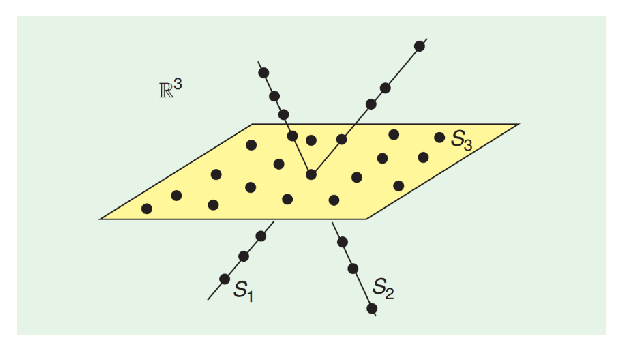
\includegraphics[width=7cm]{Matsushima/sc.eps}
    \caption{部分空間クラスタリングの3次元の例(\cite{SC}から抜粋)。距離が近い点同士ではなく、同じ平面上もしくは同じ直線上(部分空間上)にある点同士をクラスタとみなす。}
    \label{fig:my_label}
\end{figure}
\cite{HSM01}は〜\\
\cite{HSM02}は〜\\
\cite{KM01}は〜\\
\cite{KM02}は〜\\
\cite{NM01}は〜

\begin{thebibliography}{9}
\bibitem{F}
    Friedman, J., Hastie, T., & Tibshirani, R. (2010). 
    Applications of the lasso and grouped lasso to the estimation of sparse graphical models (pp. 1-22). Technical report, Stanford University.
\bibitem{SC}
 VIDAL, René. Subspace clustering. IEEE Signal Processing Magazine, 2011, 28.2: 52-68.
\end{thebibliography}



\subsection{研究報告(姜)}
\subsection{野生動物ワイヤレスセンサネットワーク実証実験基盤構築に向けた研究(川瀬)}
\subsubsection{概要}
インフラ基盤のない野生環境下での運用を想定した野生動物装着型ワイヤレスセンサネットワーク(WSN)の開発を念頭に、放牧下の家畜動物による効率的な評価実験基盤の構築を目指している。2020年度は国内の放牧場に協力を依頼し、実験基盤の構築・設置、現地での評価実験実施を目指して進めてきたが、コロナ禍により中断している。また野生動物装着型WSNに特化したデータ共有手法について検討を進めている。
\subsubsection{内容}
放牧下の家畜動物たちがモバイルセンサを持ち歩き、単独行動時に取得したデータを集団行動時に共有する。そして最終的にシンクノード付近に滞在する個体からデータを回収し、モバイル通信を介して遠隔地でデータを蓄積・リアルタイムでの分析を一体的に試みることを目指す。既に、野生動物装着型WSNを見据えた動物装着モバイルセンサノードの開発・実験、モバイル通信による広域データ収集基盤の試運転を行ってきた。そこで、本研究では放牧場及び放牧家畜の協力のもと、一体的な評価実験基盤の構築及び評価実験を実施する。
\subsubsection  {成果報告}
本研究は、2020年度国立情報学研究所公募型共同研究として進められた。北海道安平町や岩手県久慈市などの肉牛放牧場らと実験基盤の構築・設置、現地での評価実験実施の交渉を行っていたが、コロナ禍により中断している。また、野生動物装着型WSNでは、いつ・どの組み合わせで発生するかわからない野生動物同士の遭遇を考慮したうえで、無線通信での効率的かつ精確なデータ共有手法が必要になる。そこで、このデータ共有手法について検討を進めている。


\section{成果要覧}

\begin{招待講演}{1}


\end{招待講演}

\begin{招待論文}{1}


\end{招待論文}

\begin{受賞}{1}

\bibitem{SatoruNakamura201} 
小風尚樹, 中村覚, 永崎研宣:
 情報処理学会 人文科学とコンピュータシンポジウム「じんもんこん2019」 学生奨励賞 構造化記述された財務記録史料データの分析手法の開発:イギリスの船舶解体業を事例に
\end{受賞}

\begin{著書}{1}

\bibitem{SatoruNakamura301} 
中村覚(担当:共編者(共編著者)):
 デジタルアーカイブ・ベーシックス 2:災害記録を未来に活かす, 2019年8月 (ISBN: 9784585202820)
\end{著書}

\begin{雑誌論文}{1}

\bibitem{JIANG1901}
Zipei Fan, Xuan Song, Renhe Jiang, Quanjun Chen, and Ryosuke Shibasaki:
Decentralized Attention-based Personalized Human Mobility Prediction, Proceedings of the ACM on Interactive Mobile Wearable and Ubiquitous Technologies, Vol.3, No.4, pp1-26, December 2019.
\bibitem{JIANG2001}
Zipei Fan, Xuan Song, Quanjun Chen, Renhe Jiang, Ryosuke Shibasaki, and Kota Tsubouchi:  
Trajectory fingerprint: one-shot human trajectory identification using Siamese network, CCF Transactions on Pervasive Computing and Interaction, 2(2), 113-125, 2020.
\bibitem{JIANG2002}
Renhe Jiang, Quanjun Chen, Zekun Cai, Zipei Fan, Xuan Song, Kota Tsubouchi, and Ryosuke Shibasaki: 
Will You Go Where You Search? A Deep Learning Framework for Estimating User Search-and-Go Behavior, Neurocomputing, 2020.
\bibitem{JIANG2003}
Renhe Jiang, Xuan Song, Zipei Fan, Tianqi Xia, Zhaonan Wang, Quanjun Chen, Zekun Cai, and Ryosuke Shibasaki: 
Transfer Urban Human Mobility via POI Embedding over Multiple Cities, ACM/IMS Trans. Data Sci. 2, 1, Article 4, 26 pages, January 2021.
\bibitem{LMY01}
T. Lee, S. Matsushima, K. Yamanishi: “Grafting for combinatorial binary model using frequent itemset mining,” Data Mining and Knowledge Discovery, 34(1), pp. 101-123 (2020)
\bibitem{FMY01}
Y. Fu, S. Matsushima, K. Yamanishi: “Model Selection for Non-Negative Tensor Factorization with Minimum Description Length,” Entropy 2019, 21, 632.
	
\end{雑誌論文}

\begin{査読付}{1}

\bibitem{JIANG1902}
Renhe Jiang, Xuan Song, Dou Huang, Xiaoya Song, Tianqi Xia, Zekun Cai, Zhaonan Wang, Kyoung-Sook Kim, and Ryosuke Shibasaki:
Deepurbanevent: A system for predicting citywide crowd dynamics at big events, Proceedings of The 25th ACM SIGKDD International Conference on Knowledge Discovery \& Data Mining (KDD'19), pp2114-2122, July 2019.
\bibitem{JIANG1903}
Zipei Fan, Quanjun Chen, Renhe Jiang, Ryosuke Shibasaki, Xuan Song, and Kota Tsubouchi:
Deep Multiple Instance Learning for Human Trajectory Identification, Proceedings of the 27th ACM SIGSPATIAL International Conference on Advances in Geographic Information Systems (SIGSPATIAL'19), pp512-515, November 2019.
\bibitem{JIANG1904}
Xiaodan Shi, Xiaowei Shao, Zipei Fan, Renhe Jiang, Haoran Zhang, Zhiling Guo, Guangming Wu, Wei Yuan, and Ryosuke Shibasaki:
Multimodal Interaction-Aware Trajectory Prediction in Crowded Space, Proceedings of The Thirty-Fourth AAAI Conference on Artificial Intelligence (AAAI'20), pp11982-11989, February 2020.
\bibitem{JIANG2004}
Satoshi Miyazawa, Xuan Song, Renhe Jiang, Zipei Fan, Ryosuke Shibasaki, and Taisei Sato:
City-Scale Human Mobility Prediction Model by Integrating Gnss Trajectories and Sns Data Using Long Short-Term Memory, ISPRS Annals of the Photogrammetry, Remote Sensing and Spatial Information Sciences, Volume V-4-2020, 2020, pp.87-94, August 2020.
\bibitem{JIANG2005}
Quanjun Chen, Renhe Jiang, Chuang Yang, Zekun Cai, Zipei Fan, Kota Tsubouchi, Xuan Song, Ryosuke Shibasaki: 
DualSIN: Dual Sequential Interaction Network for Human Intentional Mobility Prediction, Proceedings of the 28th International Conference on Advances in Geographic Information Systems (SIGSPATIAL '20), pp.283–292, November 2020.
\bibitem{JIANG2006}
Xiaodan Shi, Xiaowei Shao, Guangming Wu, Haoran Zhang, Zhiling Guo, Renhe Jiang, Ryosuke Shibasaki: 
Social-DPF: Socially acceptable distribution prediction of futures, Proceedings of The Thirty-Fifth AAAI Conference on Artificial Intelligence (AAAI'21), February 2021.
\bibitem{HSM02}
S. Hayashi, M. Sugiyama, S. Matsushima: “Coordinate Descent Method for Log-linear Model on Posets,”  In Proceedings of IEEE International Conference on Data Science and Advanced Analytics (DSAA), pp. 99-108 (2020)
\bibitem{MB01}
S. Matsushima, M. Brbić: “Selective Sampling-based Scalable Sparse Subspace Clustering,” Advances in Neural Information Processing Systems (NeurIPS). pp. 12416-12425 (2019)
\bibitem{RSMZYV01}
P. Raman, S. Srinivasan, S. Matsushima, X. Zhang, H. Yun, S. V. N. Vishwanathan: “Scaling Multinomial Logistic Regression via Hybrid Parallelism,” ACM SIGKDD Conference on Knowledge Discovery and Data Mining (KDD), pp. 1460-1470 (2019)

\bibitem{SatoruNakamura401} 
中村覚, 佐治奈通子, 永崎研宣:
 TEI とIIIF をベースとしたオン/オフライン併合型史料研究支援システムの開発 - オスマン・トルコ語文書群を対象として,  じんもんこん2019論文集 2019 pp.293-300 2019.

\bibitem{SatoruNakamura402} 
小風尚樹, 中村覚, 永崎研宣:
 構造化記述された財務記録史料データの分析手法の開発:イギリスの船舶解体業を事例に,  じんもんこん2019論文集 2019 pp.183-190 2019.

\bibitem{SatoruNakamura403} 
Satoru Nakamura, Kazuhiro Okada, Kiyonori Nagasaki:
 An Attempt of Dissemination of TEI in a TEI-underdeveloped country: Activities of the SIG EAJ,  The 19th annual Conference and Members Meeting of the Text Encoding Initiative Consortium 2019.

\bibitem{SatoruNakamura404} 
Kazuhiro Okada, Satoru Nakamura, Kiyonori Nagasaki:
 An Encoding Strategic Proposal of “Ruby” Texts: Examples from Japanese Texts,  The 19th annual Conference and Members Meeting of the Text Encoding Initiative Consortium 2019.

\bibitem{SatoruNakamura405} 
Satoru Nakamura:
 Approach to develop Digital Collection for Small Organization considering Sustainability and Reusability with IIIF and Static File,  The 9th International Conference of Japanese Association for Digital Humanities pp.76-78 2019.

\end{査読付}

\begin{公開}{1}

\end{公開}

\begin{特許}{1}


\end{特許}

\begin{発表}{1}

\bibitem{KM01} 上月正貴、松島慎「二変数間の相互作用を考慮した一般化加法モデルの効率的な学習」第22回情報論的学習理論ワークショップ、名古屋、2019年11月
\bibitem{HSM01} 林翔太、杉山麿人、松島慎「半順序構造上の対数線形モデルのための座標降下法」第22回情報論的学習理論ワークショップ、名古屋、2019年11月
\bibitem{NM01} 西本洋紀、松島慎「対数線形モデルを基とした生成的分類器と識別的分類器のロジスティック汎化誤差の収束の比較」第23回情報論的学習理論ワークショップ、オンライン、2020年11月
\bibitem{KM02} 上月正貴、松島慎「二変数間相互作用を考慮した一般化加法モデルとその効率的な学習」科研費シンポジウム機械学習・統計学・最適化の数理とAI技術への展開、オンライン、2020年12月
\bibitem{SatoruNakamura701} 
中村覚, 水野遊大, 稗方和夫, 成田健太郎:
 デジタル文化資料活用システムの設計手法 ―法帖研究支援の事例― ,  人工知能学会研究会資料 SIG-KST-039-02 pp.1-6 2020.

\bibitem{SatoruNakamura702} 
NAKAMURA Satoru:
 Development of Content Retrieval System of Scrapbook “Kunshujo” using IIIF and Deep Learning,  2019 IIIF Conference 2019.

\bibitem{SatoruNakamura703} 
NAKAMURA Satoru, NAGASAKI Kiyonori:
 IIIF Discovery in Japan,  2019 IIIF Conference 2019.

\bibitem{SatoruNakamura704} 
佐治奈通子, 中村覚:
 歴史学と情報学のより良い協働を目指して―オープンなDH支援ツールを用いたボスニアのカトリック修道院所蔵のオスマン・トルコ語文書群のデータ整理の一事例,  研究報告人文科学とコンピュータ(CH) 2019-CH-120(11) pp.1-7 2019.

\bibitem{SatoruNakamura705} 
Ayano Kokaze, Satoru Nakamura, Kiyonori Nagasaki, Naoki Kokaze:
 Enriching the Life Cycle of data: Supporting a project by DH approach,  International Society for Eighteenth-Century Studies Congress 2019 2019.

\end{発表}

\begin{特記}{1}

\end{特記}

\begin{報道}{1}


\end{報道}


\end{document}
